\chapter{Subset sum Reconfiguration}
The subset sum problem is a well-known \NP-complete problem in which given an integer $x$ and a set of integers $S = \{a_1, a_2,\dots, a_n\}$,
we wish to find a subset $A \subseteq [n]$ such that $\sum_{i \in A} a_{i} = x$.

In \cite{Ito11approximabilityof}, Ito and Demaine considered the following problem :
Given two \textit{packings}\footnote{Please refer to \cite{Ito11approximabilityof} for the definition of packings} $A_1$ and $A_2$, both of total
size at least $k$, can we transform $A_1$ into $A_2$ via packings by moving (namely, either adding or removing) a
single item to/from the previous one without ever going through a packing of total size less than $k$. This problem is referred to as the
SUBSET SUM RECONFIGURATION problem and is proved to be strongly $\NP$-hard, and $\PSPACE$-complete for the variant with conflict graph
\cite{Ito11approximabilityof}.

In this chapter, we explore another reconfiguration version of the subset sum problem referred to as the $k$-move Subset Sum reconfiguration
problem presented in \cite{cardinal_reconfiguration_2018}. We say that a set of integers $A_1$ can be \textit{$k$-move reconfigured} into a
second set of integers $A_2$ whenever the symmetric difference of $A_1$ and $A_2$ has cardinality at most $k$. It turns out that the
$k$-move Subset Sum reconfiguration problem is $\PSPACE$-complete \cite{cardinal_reconfiguration_2018}. This chapter is dedicated to this
result. 

\textit{Roadmap.} \todo{To finish at the end}
particular proof in an attempt to detail the hardness proof.

\section{$k$-move Subset Sum Reconfiguration}
To begin our journey to the hardness proof of the $3$-move subset sum reconfiguration problem, we first start by defining the decision
problem of the $k$-move subset sum reconfiguration.
\begin{defn}{($k$-move Subset Sum Reconfiguration Problem).} Given two solutions $A_1$ and $A_2$ to an instance of the subset sum problem,
can $A_2$ be obtained by repeated $k$-move reconfiguration, beginning with $A_1$, so that all intermediate subsets are also solutions?
\end{defn}

Notice that the reconfiguration problem is trivial if the reconfiguration steps are restricted to involve only the removal or addition of a single element
of $S$, as no single such move can maintain the same sum. The problem remains trivial for $k=2$, since any removed element must be replaced by
itself. For $k=3$, the following theorem is proved:
\begin{theorem}The $3$-move Subset Sum Reconfiguration problem is strongly $\PSPACE$-complete.\end{theorem} \label{theorem:3_move}


The proof of theorem \ref{theorem:3_move} is organised in the following way : We first start by proving the membership of the $k$-move subset
sum reconfiguration problem in $\PSPACE$ (lemma \ref{lemma:k_move_pspace}). Proving the hardness is done in two steps. The first step
consists of reducing the labelled Sliding Token Reconfiguration problem to the Exact Cover Reconfiguration problem (lemma \ref{lemma:ECR}).
However before diving into the proof of lemma \ref{lemma:ECR}, we first take a detour to sections \ref{sec:sliding_problem} and
\ref{sec:Exact_cover} where the labeled sliding token reconfiguration and exact cover reconfiguration problems are introduced respectively.

The second step involves reducing the Exact Cover Reconfiguration problem to the $3$-move Subset Sum Reconfiguration problem
(theorem \ref{theorem:3_move_theorem}).

\begin{lemma}For every $k \in \mathbb{N}$, the $k$-move Subset Sum Reconfiguration problem is in $\PSPACE$. \end{lemma} \label{lemma:k_move_pspace}
\begin{proof}
For an instance with $|S| = n$, there are $O(n^{k})$ other subsets reachable by a $k-$move reconfiguration, since each such move can be specified
by the set of items in the symmetric difference of the two subsets. So all adjacent subsets in the reconfiguration graph can be enumerated in
polynomial time. Then the $k$-move subset sum reconfiguration problem is in $\NPSPACE$ by the following algorithm : in the reconfiguration graph,
repeatedly move between subsets by  non-deterministically selecting a neighbour in polynomial time and space. Since \NPSPACE $=$ \PSPACE
\cite{savitch_relationships_1970}, the $k$-move subset sum is also in $\PSPACE$.
\end{proof}


\section{Labelled SLIDING TOKEN problem.}\label{sec:sliding_problem}
The Sliding token problem is introduced in chapter \ref{chap:NCL} and detailed in section \ref{sec:sliding_tokens}. Hearn and Demaine proved that
the SLIDING TOKEN PROBLEM is $\PSPACE$-complete for planar graphs \cite{hearn_pspace-completeness_2004}, as an example of the application of
the nondeterministic constraint logic model and they implicitly proved that the SLIDING TOKEN PROBLEM is $\PSPACE$-hard on $3$-regular graphs
since the reduction is done from a restricted NCL machine (NCL-CONFIGURATION-TO-EDGE) in which the underlying graph is planar and all vertices
have degree three. The labelled variant of the sliding token problem, where each token has a unique label, is also $\PSPACE$-hard and is proved
in section \ref{sec:labeled_sliding_token} of chapter \ref{chap:NCL}.

\section{Exact Cover Reconfiguration problem} \label{sec:Exact_cover}
The exact cover reconfiguration problem is the second problem introduced along this reduction. It will be referred to as the
ECR problem throughout the rest of this thesis. The variant of the ECR problem considered here is the Exact cover split and merge
reconfiguration defined as follows :

\begin{defn}{(Exact Cover Split and Merge Reconfiguration).} Given a set $\mathcal{S}$ of subsets of a set $\mathcal{U}$, and two exact covers
$C_1$ and $C_2 \subseteq \mathcal{S}, C_1$ can be reconfigured into $C_2$ via a split (and $C_2$ can be reconfigured into $C_1$ via a merge)
provided that there exist $S_1, S_2, S_3 \subseteq \mathcal{S}$ with $C_1 - C_2 = S_1$ and $C_2 - C_1 = \{s_2, s_3\}$.

Since $C_1, C_2$ are exact covers it is mandatory that $S_1 = S_2 \cup S_3$ and $ S_2 \cap S_3 = \emptyset$.
\end{defn}

Thus, the ECR decision problem can be reformulated as follows :
\begin{defn}{(Exact Cover Reconfiguration problem).} Given a set $\mathcal{S}$ of subsets of a set $\mathcal{U}$, and two configuration
$C_1$ and $C_2$, can $C_1$ be reconfigured into $C_2$ via repeated splits and merges ?
\end{defn}

\begin{example}
Let $\mathcal{U} = \{1,2,3\}$ and $\mathcal{S} = \{\{1\}, \{2\}, \{3\}, \{1,2\}, \{2,3\}\}$ and the two given configurations be the
following : $C_1 = \{\{1\}, \{2,3\}\}$ and $C_2 = \{\{1,2\}, \{3\}\}$. A solution would be the following :

\begin{figure}[H]
\begin{center}
\begin{scaletikzpicturetowidth}{\textwidth}
\begin{tikzpicture}[scale=1]
  \node (1) [draw, rectangle] {\{\{1\}, \{2,3\}\}};
  \node (2) [below=of 1, draw, rectangle] {\{\{1\}, \{2\},\{3\}\}};
  \node (3) [below=of 2, draw, rectangle] {\{ \{1,2\}, \{3\} \}};
  \draw[->]  (1) to node [auto] {split} (2);
  \draw[->]  (2) to node [auto] {merge} (3);
\end{tikzpicture}
\end{scaletikzpicturetowidth}
\end{center}
\caption{Reconfiguration sequence which transforms $C_1$ into $C_2$ via splits and merges.}\label{fig:exact_cover}
\end{figure}
\end{example}

\subsection{$k$-colorability}
Recall that a set $\mathcal{S}$ of subsets of a set $U$ can be considered as a hypergraph $H = (U, \mathcal{S})$, where each element
of $U$ is a vertex and each element of $\mathcal{S}$ is a hyperedge. We say that a hypergraph is $k$-colorable whenever we
can assign one of $k$ colors to each vertex such that no two vertices in a hyperedge have the same color. The colourability of the ECR
problem is introduced for further use.

\subsection{$\PSPACE$-hardness result of the ECR problem.} \label{subsection:ECR_problem}
In this section we prove the hardness result of the ECR problem as the first step in order to prove theorem \ref{theorem:3_move}. This is done
by reducing the labelled variant of the SLIDING TOKEN PROBLEM to the Exact Cover Reconfiguration problem as mentioned earlier.

The proof is structured in the following way : First the input instance of the labelled sliding token reconfiguration problem is presented in
section \ref{subsubsection:input_instance}, followed by the definition of some terms used in the reduction proof in section 
\ref{subsubsection:prelim}. The output instance is described in section \ref{subsubsection:output_instance}.
Sections \ref{subsubsection:high_level} to \ref{subsubsection:23_colorability} are devoted to the proof.

\begin{lemma}The Exact Cover Reconfiguration problem is $\PSPACE$-hard for instances that are $23$-colorable hypergraphs. \end{lemma} \label{lemma:ECR}
\begin{proof}Labeled variant of the SLIDING TOKEN PROBLEM $\leq_p$ Exact Cover Reconfiguration problem.

\subsubsection{Input instance of the Labeled SLIDING TOKEN PROBLEM}\label{subsubsection:input_instance}
\begin{itemize}
  \item $G = (V,E)$, a $3$-regular graph.
  \item $T$, a set of labeled tokens.
  \item $p_1 : T \rightarrow V,$ a function mapping each labeled token to a vertex placement in the starting configuration of the output instance.
  \item $p_2 : T \rightarrow V,$ a function mapping each labeled token to a vertex placement in the ending configuration of the output instance.
  \item $I_1 = \{p_1(t) : t \in T\}$ and $I_2 = \{p_2(t) : t \in T\}$ are independent sets of size $|T| \leq |V|$.
\end{itemize}

\begin{example}{Input instance of the Labeled SLIDING TOKEN PROBLEM}
  \begin{figure}[H]
    \begin{center}
      \begin{scaletikzpicturetowidth}{\textwidth}
        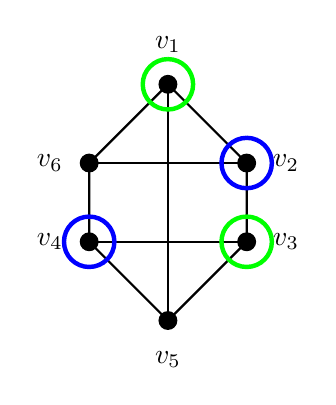
\begin{tikzpicture}[scale=1]

          \def\ver{0.12} %size of a vertex
          \def\xa{1}
          \def\ya{5}
%nodes
          \path[fill] (\xa,\ya) circle (\ver);       % v5
          \path[fill] (\xa+1,\ya+1) circle (\ver);   % v3
          \path[fill] (\xa+1,\ya+2) circle (\ver);   % v2
          \path[fill] (\xa,\ya+3) circle (\ver);     % v1
          \path[fill] (\xa-1,\ya+2) circle (\ver);   % v6
          \path[fill] (\xa-1,\ya+1) circle (\ver);   % v4
%labels
          \node (1) at (\xa,\ya+3.5) {$v_1$};     % v1
          \node (2) at (\xa+1.5,\ya+2) {$v_2$};   % v2
          \node (3) at (\xa+1.5,\ya+1) {$v_3$};   % v3
          \node (5) at (\xa,\ya-0.5) {$v_5$};     % v5
          \node (4) at (\xa-1.5,\ya+1) {$v_4$};   % v4
          \node (6) at (\xa-1.5,\ya+2) {$v_6$};   % v6
%edges
          \draw[thick] (\xa,\ya)--(\xa+1,\ya+1)--(\xa+1,\ya+2)--(\xa,\ya+3)--(\xa-1,\ya+2)--(\xa-1,\ya+1)--(\xa,\ya) ; % contour
          \draw[thick] (\xa,\ya)--(\xa,\ya+3) ;       % v5 - v1
          \draw[thick] (\xa+1,\ya+1)--(\xa-1,\ya+1) ; % v3 - v4
          \draw[thick] (\xa+1,\ya+2)--(\xa-1,\ya+2) ; % v2 - v6
%independent sets
          \draw[ultra thick,green] (\xa,\ya+3+ \ver+0.2) coordinate(a1)  arc (90:450:\ver +0.2) coordinate(a2);
          \draw[ultra thick,green] (\xa+1,\ya+1+ \ver+0.2) coordinate(d1)  arc (90:450:\ver +0.2) coordinate(d2);
          \draw[ultra thick,blue] (\xa-1,\ya+1+ \ver+0.2) coordinate(a1)  arc (90:450:\ver +0.2) coordinate(a2);
          \draw[ultra thick,blue] (\xa+1,\ya+2+ \ver+0.2) coordinate(d1)  arc (90:450:\ver +0.2) coordinate(d2);

        \end{tikzpicture}
      \end{scaletikzpicturetowidth}
    \end{center}
    \caption{A $3$-regular graph $G=(V,E)$ and initial independent set $I_1 = \{v_1, v_3\}$}
    \label{fig:input_sliding_token_example}
  \end{figure}
\end{example}

\subsubsection{Preliminaries} \label{subsubsection:prelim}
Before diving in the proof, a few concepts that will be used are presented hereunder :
\paragraph{Slide Set.}
For each pair of adjacent vertices $v_i, v_j \in V$ of the input instance of the sliding token problem, the set consisting of these two vertices
and their neighbors is called a $slide set$, denoted $S_{i,j}$.
\begin{figure}[H]
  \begin{center}
    \begin{scaletikzpicturetowidth}{\textwidth}
      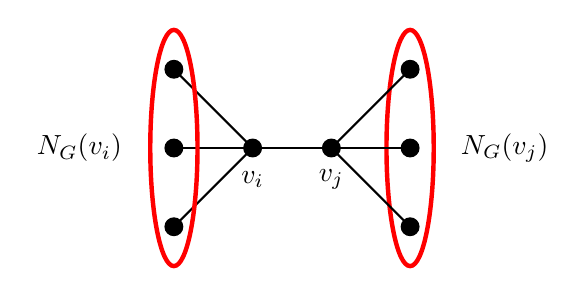
\begin{tikzpicture}[scale=1]
      \def\ver{0.12} %size of a vertex
      \def\x{1}
      \def\xa{1}
      \def\ya{0}
      \def\xb{2}
      %Slide Set
      \path[fill] (\xa,\ya) circle (\ver);       % vi
      \node (1) at (\xa,\ya-0.4) {$v_i$};
      \path[fill] (\xa-1,\ya) circle (\ver);     % v2
      \path[fill] (\xa-1,\ya+1) circle (\ver);   % v1
      \path[fill] (\xa-1,\ya-1) circle (\ver);   % v3

      \draw[thick] (\xa,\ya)--(\xa-1,\ya) ;
      \draw[thick] (\xa,\ya)--(\xa-1,\ya+1) ;
      \draw[thick] (\xa,\ya)--(\xa-1,\ya-1) ;
      \draw[ultra thick, red] (0,0) ellipse (0.3 and 1.5);
      \node (3) at (\xa-2.2,\ya) {$N_{G}(v_i)$};
      \draw[ultra thick, red] (3,0) ellipse (0.3 and 1.5);
      \node (3) at (\xb+2.2,\ya) {$N_{G}(v_j)$};

      %graph independent set
      \path[fill] (\xb,\ya) circle (\ver);       % v_j
      \node (1) at (\xb,\ya-0.4) {$v_j$};
      \path[fill] (\xb+1,\ya) circle (\ver);    % v2
      \path[fill] (\xb+1,\ya+1) circle (\ver);   % v1
      \path[fill] (\xb+1,\ya-1) circle (\ver);   % v3
      \draw[thick] (\xb,\ya)--(\xb+1,\ya) ;
      \draw[thick] (\xb,\ya)--(\xb+1,\ya+1) ;
      \draw[thick] (\xb,\ya)--(\xb+1,\ya-1) ;

      \draw[thick] (\xa,\ya)--(\xb,\ya) ;
      \end{tikzpicture}
    \end{scaletikzpicturetowidth}
  \end{center}
  \caption{Slide set denoted $S_{ij}$ of vertices $v_i$ and $v_j$.}
  \label{fig:slide_set}
\end{figure}

\paragraph{Maximally split configuration $C$.}
A configuration $C$ of the output Exact Cover instance is called \textit{maximally split} if every $c \in C$
contains exactly one vertex and up to one token.

\begin{example}{A maximally split configuration $C$}
  \begin{figure}[h!]
    \begin{center}
      \begin{scaletikzpicturetowidth}{\textwidth}
        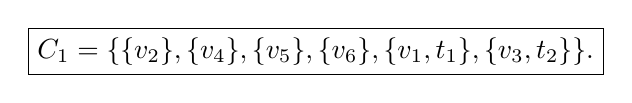
\begin{tikzpicture}[scale=1]
          \node (1) [draw, rectangle] {$C_1 = \{ \{v_2\}, \{v_4\}, \{v_5\}, \{v_6\}, \{v_1, t_1\}, \{v_3, t_2\} \}$.};
        \end{tikzpicture}
      \end{scaletikzpicturetowidth}
    \end{center}
    \caption{A maximally split configuration $C_1$.}
    \label{}
  \end{figure}
\end{example}

\paragraph{Sploot set of a configuration $C$.}
For each exact cover configuration $C$ in the output instance, let sploot($C$) be the set of all maximally split configurations reachable from $C$.


\subsubsection{Output $\mathcal{U}$ and $\mathcal{S}$}\label{subsubsection:output_instance}
The output instance of the Exact Cover Reconfiguration problem contains a set $\mathcal{S}$ of subsets of a set $\mathcal{U}$ defined in
\ref{sec:Exact_cover} where :
\begin{itemize}
  \item $\mathcal{U} = \{v_1, v_2, \dots, v_{|V|}\} \cup \{t_1, t_2, \dots, t_{|T|}\}.$
  \item The set $\mathcal{S}$ is defined as follows, for every pair of adjacent vertices $v_i, v_j$ and token $t_k$
    \begin{itemize}
      \item All subsets of $S_{i,j} - \{v_i\}$ and $S_{i,j} - \{v_j\}$.
      \item $\{v_i, t_k\}$ and $\{v_j , t_k\}$.
      \item $S_{i,j} \cup \{t_k\}$.
    \end{itemize}
\end{itemize}

\begin{example}According to the above example, \ref{fig:input_sliding_token_example}, the output instance of the Exact Cover Reconfiguration
problem is the following : \todo{Do the output instance in tikz}
\end{example}

\subsubsection{Output exact cover starting and ending configurations, $C_1$ and $C_2$}
The starting configuration $C_1$ is the union of $\{\{ v_i \} : v_i \in V - I_1\}$ and, for every $v_i \in I_1$, a set $\{v_i, t_k\}$ with a
distinct $t_k$.
The ending configuration $C_2$ is then the union of $\{\{ v_i \} : v_i \in V - I_2\}$ and, for every $v_i \in I_2$, a set $\{v_i, t_k\}$ with a
distinct $t_k$.

\begin{example}Continuing the running example, $C_1$ and $C_2$ would be :
\begin{itemize}
  \item $C_1 = \{ \{v_2, v_4, v_5, v_6\}, \{v_1, t_1\}, \{v_3, t_2\}\}$.
  \item $C_2 = \{ \{v_1, v_3, v_5, v_6\}, \{v_2, t_1\}, \{v_4, t_2\}\}$.
\end{itemize}
\end{example}

\subsubsection{$23$-colorability of the output instance $H = (U, \mathcal{S})$}\label{subsubsection:23_colorability}
The goal here is to make sure that no two vertices of distance at most $3$ (i.e. in a common slide set see figure \ref{fig:slide_set}) have the same
color. More precisely, we want to prove that given $23$-colours, no two vertices having a common slide set would have the same colour.
This constraint will enforce the absence of tokens on neighbors of $v_i$ and $v_j$, and the presence of a token on $v_i$ or $v_j$, but not both
making sure that any merge or split will result into a feasible configuration. \todo{reformulate}.

Given that the $kth$ power $G^{k}$ of an undirected graph $G$ is another graph that has the same set of vertices, but in which two vertices are
adjacent when their distance in $G$ is at most $k$, to find the colorability of the output instance $H = (U, \mathcal{S})$, it suffices to
compute $\Delta(G^{3})$. Since $G$ is $3-$regular, $G^3$ has degree at most $21$ proven by the following figure where the worst case
scenario ($i.e.,$ a tree is attached to each root so as to force the root to meet new nodes and add new edges \todo{To reformulate this correctly}).


\begin{figure} [H]
  \centering
  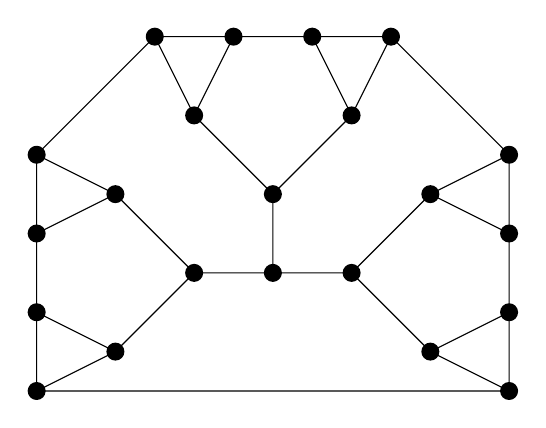
\begin{tikzpicture}
    \def\xa{0}
    \def\ya{0}
    %nodes
    \draw[thick, fill=black] (\xa,\ya) circle (0.1cm);           % v1

    \draw[thick, fill=black] (\xa+1,\ya) circle (0.1cm);         % v2
    \draw[thick, fill=black] (\xa+2,\ya+1) circle (0.1cm);       % v3
    \draw[thick, fill=black] (\xa+2,\ya-1) circle (0.1cm);       % v4
    \draw[thick, fill=black] (\xa+3,\ya-0.5) circle (0.1cm);     % v5
    \draw[thick, fill=black] (\xa+3,\ya-1.5) circle (0.1cm);     % v6
    \draw[thick, fill=black] (\xa+3,\ya+1.5) circle (0.1cm);     % v7
    \draw[thick, fill=black] (\xa+3,\ya+0.5) circle (0.1cm);     % v8

    \draw[thick, fill=black] (\xa,\ya+1) circle (0.1cm);         % v9
    \draw[thick, fill=black] (\xa+1,\ya+2) circle (0.1cm);       % v10
    \draw[thick, fill=black] (\xa-1,\ya+2) circle (0.1cm);       % v11
    \draw[thick, fill=black] (\xa+1.5,\ya+3) circle (0.1cm);     % v12
    \draw[thick, fill=black] (\xa+0.5,\ya+3) circle (0.1cm);     % v13
    \draw[thick, fill=black] (\xa-0.5,\ya+3) circle (0.1cm);     % v14
    \draw[thick, fill=black] (\xa-1.5,\ya+3) circle (0.1cm);     % v15

    \draw[thick, fill=black] (\xa-1,\ya) circle (0.1cm);         % v16
    \draw[thick, fill=black] (\xa-2,\ya+1) circle (0.1cm);       % v17
    \draw[thick, fill=black] (\xa-2,\ya-1) circle (0.1cm);       % v18
    \draw[thick, fill=black] (\xa-3,\ya-1.5) circle (0.1cm);     % v19
    \draw[thick, fill=black] (\xa-3,\ya-0.5) circle (0.1cm);     % v20
    \draw[thick, fill=black] (\xa-3,\ya+0.5) circle (0.1cm);     % v21
    \draw[thick, fill=black] (\xa-3,\ya+1.5) circle (0.1cm);     % v22

    %edges
    \draw (\xa,\ya)--(\xa+1,\ya)--(\xa+2,\ya-1)--(\xa+3,\ya-1.5) ;         % v1 - v2 - v4 - v6
    \draw (\xa+1,\ya)--(\xa+2,\ya+1)--(\xa+3,\ya+1.5) ;                      % v2 - v3 - v7
    \draw (\xa,\ya)--(\xa,\ya+1)--(\xa+1,\ya+2)--(\xa+1.5,\ya+3) ;     % v1 - v9 - v10 - v12
    \draw (\xa,\ya+1)--(\xa-1,\ya+2)--(\xa-1.5,\ya+3) ;            % v9 - v11 - v15
    \draw (\xa,\ya)--(\xa-1,\ya)--(\xa-2,\ya-1)--(\xa-3,\ya-1.5) ;   % v1 - v16 - v18 - v19
    \draw (\xa-1,\ya)--(\xa-2,\ya+1)--(\xa-3,\ya+1.5) ; % v16 - v17 - v22
    \draw (\xa-2,\ya-1)--(\xa-3,\ya-0.5) ; % v18 - v20
    \draw (\xa-2,\ya+1)--(\xa-3,\ya+0.5) ; % v17 - v21
    \draw (\xa-1,\ya+2)--(\xa-0.5,\ya+3) ; % v11 - v14
    \draw (\xa+1,\ya+2)--(\xa+0.5,\ya+3) ; % v10 - v13
    \draw (\xa+2,\ya+1)--(\xa+3,\ya+0.5) ;  % v3 - v8
    \draw (\xa+2,\ya-1)--(\xa+3,\ya-0.5) ; % v4 - v5

    \draw (\xa+3,\ya-1.5)--(\xa-3,\ya-1.5)--(\xa-3,\ya-0.5)--(\xa-3,\ya+0.5)--(\xa-3,\ya+1.5)--(\xa-1.5,\ya+3)--(\xa-0.5,\ya+3)--(\xa+0.5,\ya+3)--(\xa+1.5,\ya+3)--(\xa+3,\ya+1.5)--(\xa+3,\ya+0.5)--(\xa+3,\ya-0.5)--(\xa+3,\ya-1.5)--(\xa-3,\ya-1.5) ; %contour

  \end{tikzpicture}
  \caption{Graph $G^{'}$ (shown darker) is a subgraph of $G$.}
  \label{fig:subgraph}
\end{figure}


So $G$ can be $22-$colored such that no two vertices of distance at most $3$ have the same color. Coloring the tokens in $\mathcal{T}$
a distinct (23rd) color then gives a coloring of $\mathcal{U}$ such that no pair of elements of a common set share the same color.

\subsubsection{High level idea}\label{subsubsection:high_level}
We first note that the subsets containing exactly one vertex and a token (e.g., $\{v_i, t_k\}$) represents the presence of the token
$t_k$ on vertex $v_i$ and the subsets consisting of a slide set and a token (e.g., $\{S_{i,j} \cup t_k\}$) represent the presence of a
"mid-slide" token between $v_i$ and $v_j$. A "mid-slide" token can be interpreted as the token $t_k$ not being properly on $v_i$ or $v_j$ but is
"on it's way" from $v_i$ to $v_j$. Therefore, sliding a token $t_k$ from $v_i$ to $v_j$ is simulated by first
merging $\{v_i, t_k\}$ and $S_{i,j}-\{v_i\}$ into $S_{i,j} \cup \{t_k\}$, and then splitting this set into this set into $S_{i,j}-\{v_j\}$
and ${v_j, t_k}$. The first step of this sequence enforces the absence of tokens on neighbors of $v_i$ and $v_j$ since by definition, the slide
set $S_{ij}$ of $v_i$ and $v_j$ contains all the of $v_i$ and $v_j$ and having the token $t_k$  merged in $S_{ij}$ means that $t_k$ is not on any
vertex. The second step then ensures the presence of a token on $v_i$ or $v_j$, but not both.
Before a merge-split sequence, additional splits and merges of token-less sets may be needed to obtain $S_{i,j}-\{v_i\}$.

\subsubsection{Bijection between configurations.}
Given the definition of maximally split configurations in \ref{sssec:prelim}. The following defines a function $f_{red}$ from token arrangements
to maximally split covers in the following way :
\begin{enumerate}
  \item Each token-less vertex corresponds to a set $\{v_i\}$ in the cover.
  \item Each token $t_k$ placed at $v_i$ corresponds to a set $\{v_j, t_k\}$ in the cover.
\end{enumerate}
Notice that $f_{red}$ is a bijection since each cover configuration is an exact cover (pas de doublons) and each token
arrangement contains no doublons no plus. Notice also that $f_{red}(p_1) = C_1$ and $f_{red}(p_2) = C_2$.
\todo{I do not agree with f(p1) = c1 etc}

\subsubsection{Reduction structure.}
The remainder of the proof is devoted to proving the following claim:
\begin{claim} A token arrangement $p^{'}$ is reachable from a token arrangement $p$ if and only if $f_{red}(p^{'})$ is reachable from
$f_{red}(p)$ via split and merges.
\end{claim}
Both directions are proved inductively. That is, we consider only “adjacent” configurations. We also assume that the starting token
arrangement $p : T \rightarrow V$ has $ \{p(t) : t \in T \}$ independent.

\subsubsection{Sliding tokens reachability  $\rightarrow$ Exact cover reachability}
Let $p$ be a token arrangement that can be reconfigured into $p^{'}$ via a token slide from $v_i$ to $v_j$. Then $f_{red}(p^{'})$ can be reached
from $f_{red}(p)$ via the following sequence of merges and splits.
\begin{enumerate}
  \item Repeatedly merge token-less vertex sets to form $S_{i,j}-\{v_i\}$.
  \item Merge $S_{i,j} - \{v_i\}$ and $\{v_i, t_k\}$ into $S_{i,j} \cup \{t_k\}$.
  \item Split $S_{i,j} \cup \{t_k\}$ into $S_{i,j} - \{v_j\}$ and $\{v_j, t_k\}$.
  \item Repeatedly split the token-less vertex set $S_{i,j}-\{v_j\}$ into single vertex sets.
\end{enumerate}

\begin{example}A token slide from $v_1$ to $v_6$ is simulated by first merging $\{v_1, t_1\}$ and $S_{1,6} - \{v_1\}$ into $S_{1,6} \cup \{t_1\}$,
and then splitting this set into this set into $S_{1,6} - \{v_6\}$ and $\{v_6, t_1\}$.
\end{example}

\subsubsection{Exact Cover reachability $\rightarrow$ Sliding tokens reachability}\label{subsubsection:backward}

For each exact cover configuration $C$ in the output instance, let \textit{sploot(C)} be the set of all maximally split configurations reachable
from $C$. Let $C$ and $C^{'}$ be two maximally split configurations such that $C$ can be reconfigured into $C^{'}$ and $C_{inter}$ be the first
configuration encountered in the reconfiguration sequence such that \textit{sploot($C_{inter}$)} $\neq \{C\}$.

\begin{obs}
Since $C$ and $C^{'}$ are both maximally split configurations, the only way of obtaining $C_{inter}$ is by merging two sets, one of which contains
a token. Thus, $C_{inter}$ is obtained by merging $\{v_i, t_k\}$ and $S_{i,j} - \{v_i, t_k\}$  to form $S_{i,j} \cup \{t_k\}$ for
some $v_i, v_j$ and $t_k$.
\end{obs}

\begin{remark}
It may be the case for other pairs $i^{'}, j^{'}$ that $S_{i,j} = S_{i^{'}, j^{'}}$.
\end{remark}

Once $C_{inter}$ is reached two moves can be considered to move forward :
\begin{enumerate}
  \item Either split $S_{i,j} \cup t_k$ back to $S_{i,j} - \{v_i,t_k\}$ to obtain the previous configuration.
  \item Or split $S_{i,j} \cup t_k$ into $S_{i^{'},j^{'}} - \{v_j^{'},t_k\}$ where $S_{i,j} = S_{i^{'}, j^{'}}$.
\end{enumerate}

By definition of the exact cover configuration $C$, since $S_{i,j} - \{v_i\}, \{v_i, t_k\} \in C$, the token
arrangement $p$ with $f_{red}(p) = C$ has no tokens on vertices in $S_{i,j}$ except for token $t_k$ on $v_i$. Added the fact
that $S_{i,j} = S_{i^{'}, j^{'}}$, it contains all the neighbors of $v_i, v_i^{'}, v_j, v_j^{'}$. Thus the token
arrangement obtained by moving the location of $t_k$ in $p$ from $v_i$ to $v_j$, $v_i^{'}$, or $v_j^{'}$ results in an independent set because
the constraint to statisfy in order to split from $C_{inter}$ to $C^{'}$ was to split s.t $S_{i,j} = S_{i^{'}, j^{'}}$.

So all that remains is to prove that there are a sequence of slides moving $t_k$ from $v_i$ to $v_j^{'}$ via vertices
in $\{v_i, v_j, v_i^{'}, v_j^{'}\}$. Since $S_{i,j} = S_{i^{'},j^{'}}$ it means that $v_i^{'}, v_j^{'} \in S_{i,j}$ too.
So either $v_i \in {v_i^{'}, v_j^{'}}$, or there is an edge $\{v_i, v_i^{'}\}$ or $\{v_i, v_j^{'}\} \in E$. So $t_k$ can slide
from $v_i$ to either $v_i^{'}$ or $v_j^{'}$ (via 0 or 1 slides), and then from $v_i^{'}$ or $v_j^{'}$ to $v_j^{'}$ (via 0 or 1 slides).

\todo{Add simple example here to demonstrate the last part}
\end{proof}

\begin{example}{}
\end{example}

\section{$3$-move Subset Sum reconfiguration problem}

\subsection{$\PSPACE$-hardness result} \label{subsection:3_move_hardness}
\begin{theorem}{The $3$-move Subset Sum Reconfiguration problem is strongly $\PSPACE$-complete.}\end{theorem} \label{theorem:3_move_theorem}

\begin{proof}The reduction is from the Exact Cover Reconfiguration problem for instances that are $23-$colorable induced hypergraphs,
proved $\PSPACE$-hard.

\subsubsection{Input Instance of the Exact Cover Reconfiguration problem}
Recall that the Exact Cover Reconfiguration instance contains a set $\mathcal{S}$ of subsets of a set $\mathcal{U}$ and two exact
covers $C_1$ and $C_2 \subseteq \mathcal{S}$.


\subsubsection{High level idea}
Every $3-$move Subset Sum Reconfiguration step is either a \textit{merge} where $a_i$ and $a_j$ are replaced by $a_i + a_j$ or a \textit{split}
where $a_i + a_j$ is replaced by $a_i$ and $a_j$.

\subsubsection{Reduction Structure}
Given an instance of the exact cover problem, each element $a$ of $U$ is given an arbitrary label $i$ where $i \in \{1, \dots, |U|\}$ and
is partitioned according to its color $j$ where $j \in \{1, \dots, 23\}$.
A function $f : \mathcal{U} \rightarrow \mathbb{N}$ maps each element of the universe $\mathcal{U}$ of the input Exact Cover Reconfiguration
problem to a positive integer. The positive integer is computed using the encoding of the label and color of an element $a$. The function
$f$ maps a color-$j$ element $a_{i}$ to $i.2^{100j \lceil log_{2}(|U|) \rceil}$. In binary, this mapping consists of the binary encoding of
$i$ followed by $100j \lceil log_{2}(|U|) \rceil$ zeros. The idea here is to use $j$ to create an interval for elements of $U$ have the same
colour or are part of the same colour class and $i$ as an offset to differentiate elements of the same colour.


\subsubsection{Output $\mathcal{S}$ and $x$}
The numbers in the output $3-$move Subset Sum Reconfiguration instances are $\{\sum_{a \in S} f(a) : S \in \mathcal{S}\}$ and the
output target sum is $\sum_{a \in \mathcal{U}} f(a)$.

\subsubsection{Output size}



\subsubsection{Correctness}
A reconfiguration in both the exact cover and $3$-move subset sum problems involves splitting
or merging elements. Thus it suffices to prove that the function $f$ yields a one-to-one mapping $g : \mathcal{S} \rightarrow N$
given by $g(\mathcal{S}) = \sum_{a \in \mathcal{S}}^{} f(a)$.

Recall that the function $f$ maps each element $a_i \in U$ to a value based upon the color of $a_i$. The sums of
the outputs of $f$ for all elements of all colors $1$ to $j-1$ is at most $2^{100(j-1)} log_{2}(|U|)|U|^{2} \leq 2^{(100j-98)}log_{2}(|U|)$
while the output of $f$ for any element of any color $j$ or larger is at least $2^{100(j)} log_{2}(|U|) \geq 2^{(98)}log_{2}(|U|)$.

Thus if a pair of sets $\mathcal{S}_1, \mathcal{S}_2 \subseteq S$ have $\mathcal{S}_1 = \mathcal{S}_2$, then their color-$j$ elements
differ, this difference cannot be made up by adding or removing elements of colors $1$ to $j-1$ (values too small) or colors $j + 1$ to $23$
(values too large). Thus if $\mathcal{S}_1 = \mathcal{S}_2$, then $g(\mathcal{S}_1) = g(\mathcal{S}_2)$.
\todo{Demythyfy this!!!!!!!!!! + Correction needed}


\end{proof}




